\begin{figure}[H]
    \centering
    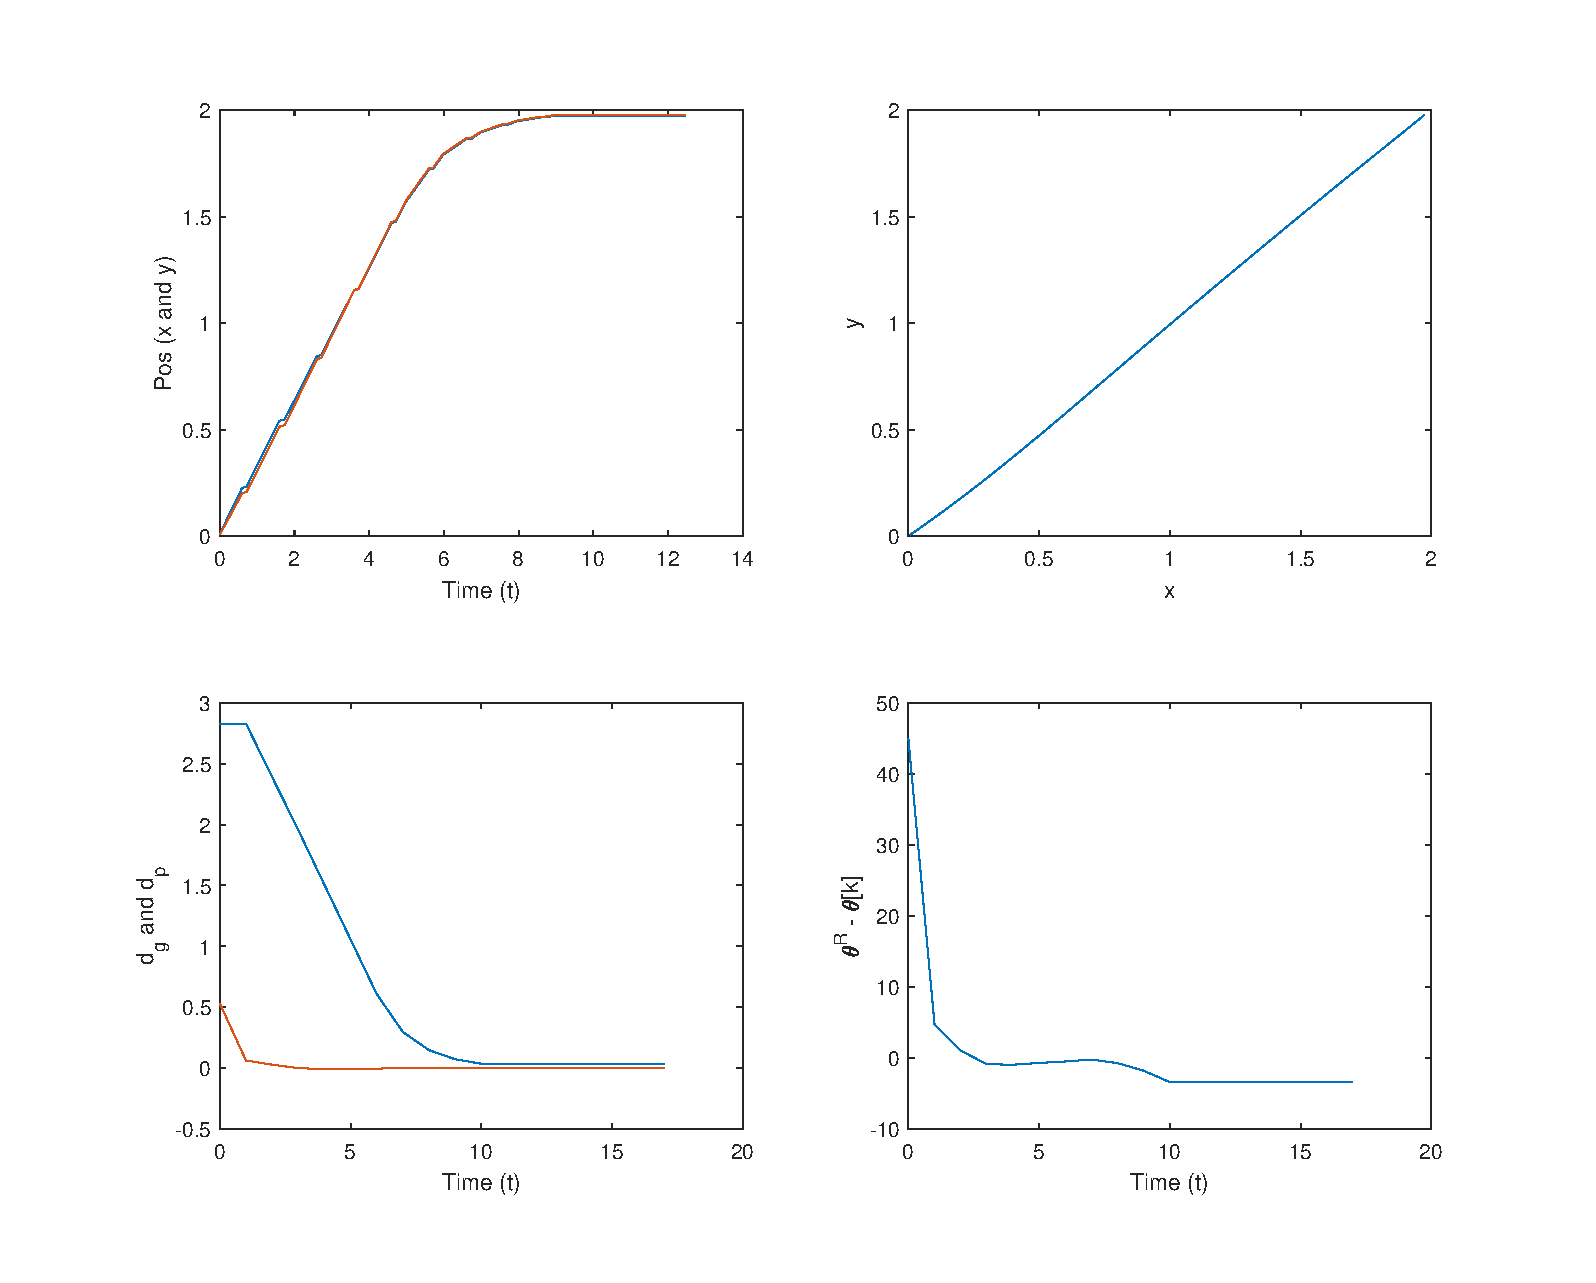
\includegraphics[width=\textwidth]{figs/perf-hybrid.eps}
    \caption{Simulation of the hybrid controller going from $(0, 0)$ to $(2, 2)$ with $K_\omega = \frac{180}{R\pi}$, and $p = 0.75.$ The directional controller has $K_\psi = \frac{L}{R}$ and the got to goal controller uses $K_\psi = \frac{180}{\pi} \frac{L}{Rp}$} \label{fig:perf-hybrid}
\end{figure}

\begin{figure}[H]
    \centering
    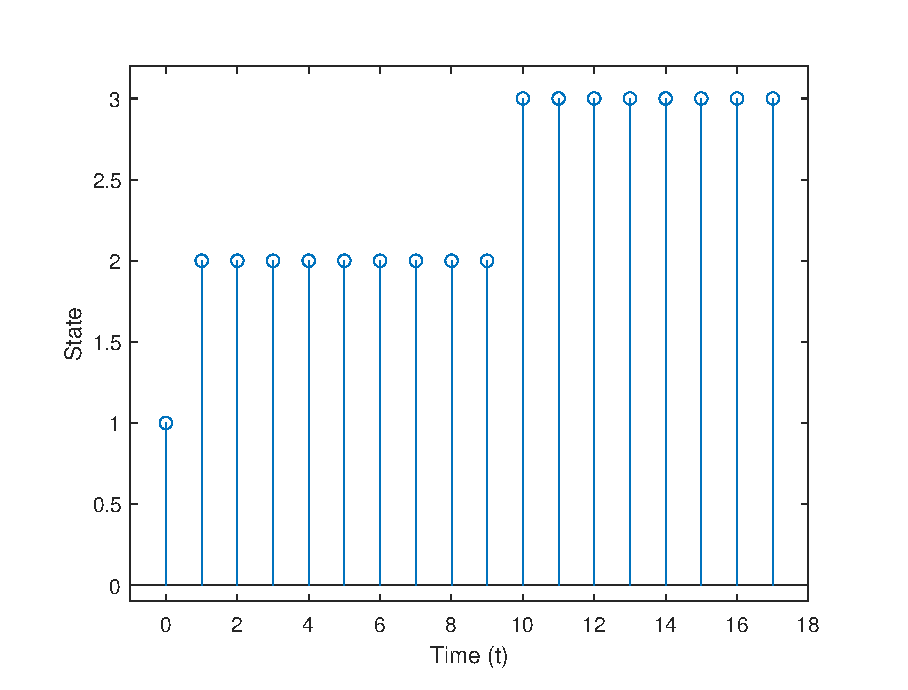
\includegraphics[width=\textwidth]{figs/state.eps}
    \caption{The sequence of discrete states of the hybrid controller going from $(0, 0)$ to $(2, 2)$ with a starting angle of 0. } \label{fig:states}
\end{figure}

The discrete state would be expected to first go into $q_1$ for a short while when the robot turns towards the direction of the goal. Then it should go into state $q_2$ for a while when driving towards the goal, and finally it should end up in state 3 when it has reached the goal. This is the exact behavior that is shown in figure \ref{fig:states}.